%==============================================================================
\chapter{Figures}
\label{sec:fig}\index{figures}
%==============================================================================

\LaTeX{} file: \url{./guide_figs.tex}\\[1ex]
\noindent
This chapter discusses what you need to know to include graphics in
your thesis. The basic command to use is \Macro{includegraphics}.

I recently found a pretty complete guide (in German) called \texttt{l2piqfaq}
which can be obtained from
\url{http://www.ctan.org/tex-archive/info/l2picfaq/german}. It contains
a lot of detailed information and tricks.

The chapter also contains some suggestions as to how to create Feynman
graphs with a number of different packages.

%------------------------------------------------------------------------------
\section{Simple figures}
\label{sec:fig:simple}
%------------------------------------------------------------------------------

A simple figure and its associated caption is straightforward to
include. For example, the layout of the LHC and its experiments is
shown in Fig.~\ref{fig:LHC}.

\begin{figure}[htbp]
  \centering
  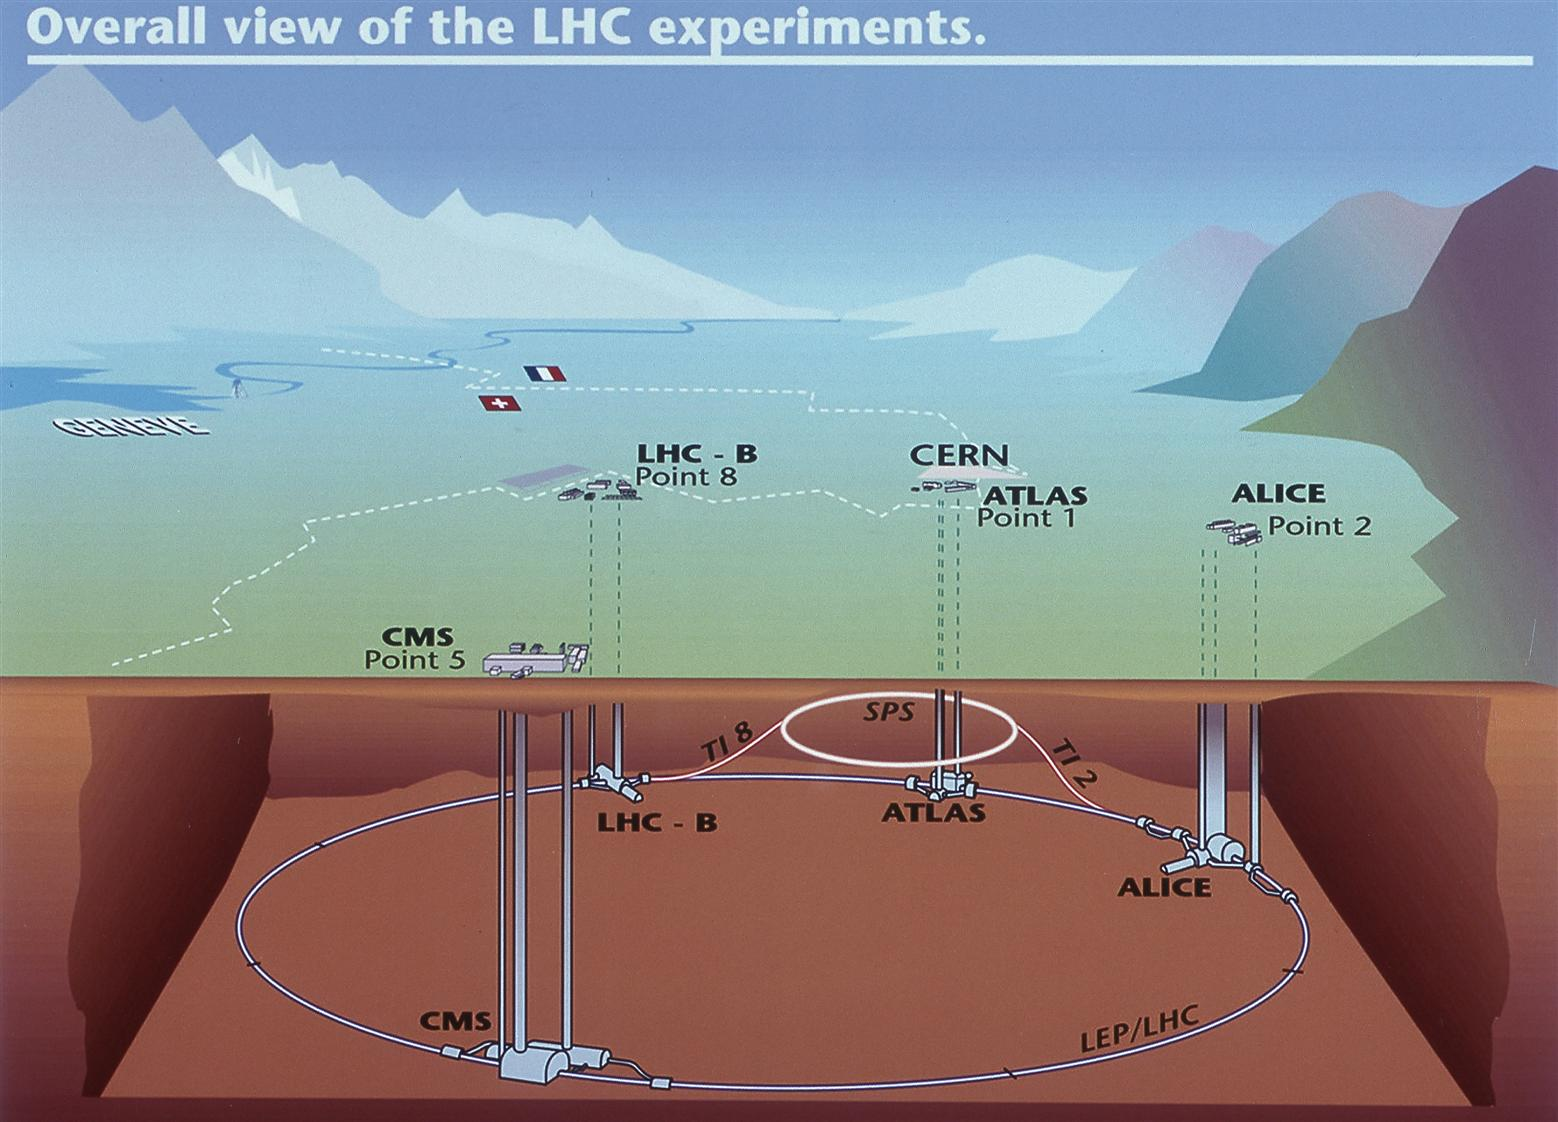
\includegraphics[width=\figwidth]{CERN_all-experiments}
  \caption[Sketch of the LHC ring, the position of the experiments and
  the surrounding countryside.]{Sketch of the LHC ring, the position
    of the experiments and the surrounding countryside. The four big
    LHC experiments are indicated. The location of the injection lines
    and the SPS are also shown.}
  \label{fig:LHC}
\end{figure}

Note the use of \Macro{centering} rather than the environment
\BegEnv{center} \ldots \EndEnv{center} to centre the figure. This
avoid adding extra vertical space. It is also important that the
\Macro{label} be either inside the caption or after it. If your
caption is more than 1 (or 2) lines, you should also give a short form
that will appear in the ``List of Figures''.

One tricky question is how to best format the caption. This document
uses a smaller font and no extra indentation. Often italics are
used. I dislike this, as symbols are then formatted in different ways
in the main text and in the caption. One can also reduce the width of
the caption. The font for the caption can be specified using the
\Macro{setkomafont}\texttt{\{caption\}} command. You can specify how
to label the figure by changing the \Macro{figureformat} command. The
captions in this document follow the standard \KOMAScript{}
convention: if they are one line long they are centred; if they are
longer they are left-adjusted. If you want them all to be
left-adjusted set the \Option{KOMAoptions} \Option{caption=nooneline}
in \texttt{ubonn-thesis.sty}. Some examples of the possibilities are
included in the style file.

Another thing to consider is whether the text should be indented or
not. For short captions, indentation is OK. I do not think it looks
good for long captions. Hence the style file sets
\Macro{setcapindent}\texttt{\{0pt\}}.

%------------------------------------------------------------------------------
\section{Fancier figures}
\label{sec:fig:fancy}\index{figures!multiple}
%------------------------------------------------------------------------------

Life gets more complicated if you want to include several plots in
one figure, if you want the caption next to the figure, or if you want
the text to \enquote{flow} around the figure. For the first case I like to
use the \Env{tabular} environment to place the plots, although
there are other ways of doing it.

Another very nice way to add (a), (b) etc. to the figure is to use the
\Macro{put} command. This has the big advantage that you can display
the letters in the figure without actually having to add them to the
EPS/PDF file. Figure~\ref{fig:letters1} shows how this is done. Note
that the origin of the coordinate system is the bottom right-hand
corner of the file that you have included (assuming that the
\Macro{put} command comes just after the \Macro{includegraphics}).
The units for the \Macro{put} command are set with the
\Macro{setlength}\texttt{\{\textbackslash unitlength\}} command, which
is by default set to \SI{1}{\mm} in \texttt{ubonn-thesis.sty}. The
same units are also used for Feynman graphs made with the
\Package{feynmf} and/or \Package{feynmp} package -- see
Section~\ref{sec:fig:feynman:feynmf}.

\begin{figure}[htbp]
  \centering
  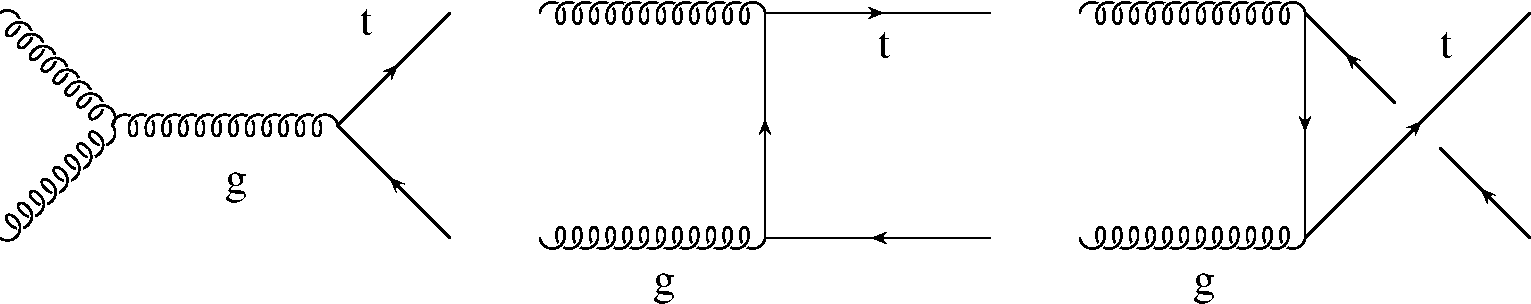
\includegraphics[width=\figwidth]{gg_tt}
  \put(-130,14){(a)}
  \put(-80,14){(b)}
  \put(-35,14){(c)}
  \caption{Adding letters to figures with \Macro{put}.}
  \label{fig:letters1}
\end{figure}

Another way of achieving the same thing, but this time with the letter
outside the figure is to use \Env{tabular}. An example of this is
shown in Fig.~\ref{fig:letters2}.

\begin{figure}[htbp]
  \centering
  \begin{tabular}{@{\hspace*{0.15\figwidth}}p{0.33\figwidth}p{0.33\figwidth}l}
    \multicolumn{3}{c}{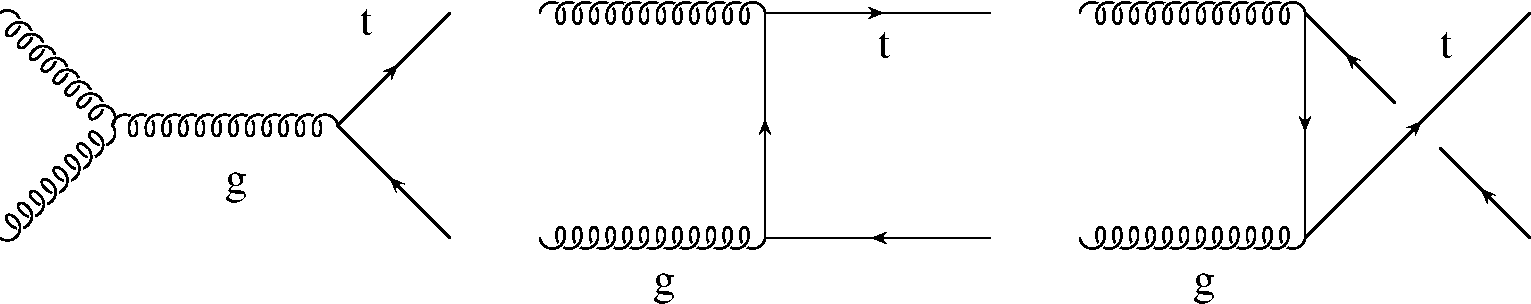
\includegraphics[width=\figwidth]{gg_tt}}\\
    (a) & (b) & (c)
  \end{tabular}
  \caption{Adding letters to figures with \Env{tabular}.}
  \label{fig:letters2}
\end{figure}

If you want to save space it is sometimes nice to put the caption next
to the figure. While packages exist to do this, \KOMAScript{} has its
own built-in \Env{captionbeside} environment. The placement option comes
after the caption itself and can be one of:
\begin{description}\setlength{\parskip}{0pt}
\item[l] Left of figure
\item[r] Right of figure
\item[i] Inner margin in two-sided layout
\item[o] Outer margin in two-sided layout
\end{description}
Note that this is an environment rather than a macro and that the
figure itself is inside the environment. Also the placement does not
seem to work exactly how it is advertised in the manual. I set the
width equal to \Macro{figwidth} and then the offset to \texttt{-\Macro*{figwidth}}.

\begin{figure}[htbp]
  \centering
  \begin{captionbeside}{A small figure with a simple caption beside it.}[i][\figwidth][-\figwidth]
    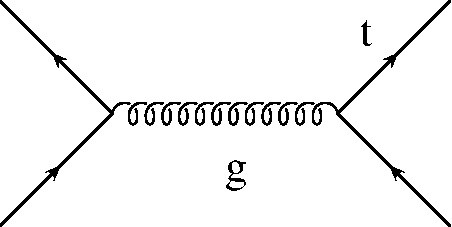
\includegraphics[width=0.3\textwidth]{qq_tt}
  \end{captionbeside}
  \label{fig:qqtt}
\end{figure}

If you want different (partial) captions for a figure then the
\Package{subfig} package used to be the way to go. You can see how to
reference the different parts of the figure in
Section~\ref{sec:fig:feynman}. If you want the captions of the
sub-figures to also appear in the \enquote{List of Figures} you should
include the package with the option \Option{lofdepth}. For tables use
the option \Option{lotdepth}.

An alternative, and successor, to \Package{subfig} is
\Package{subcaption}. It works in much the same way as
\Package{subfig}. A nice tutorial on its use can be found in
\url{http://www.peteryu.ca/tutorials/publishing/latex_captions}

\begin{figure}[htbp]
  \centering
  \subfloat[NC scattering][NC]{\label{fig:nccc-nc}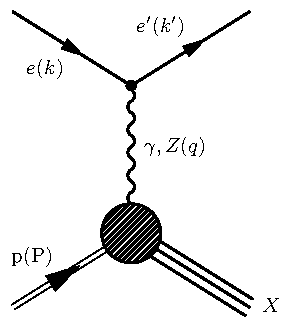
\includegraphics[width=0.5\figwidth]{ep_nc}}
  \qquad
  \subfloat[CC scattering][CC]{\label{fig:nccc-cc}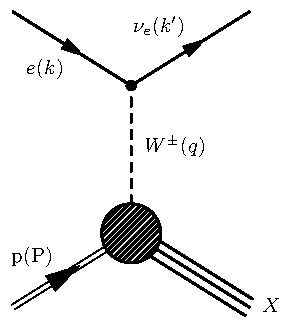
\includegraphics[width=0.5\figwidth]{ep_cc}}
  \caption{Processes in $ep$ scattering.}
  \label{fig:nccc}
\end{figure}

If you run out of space (applies more often to proceedings than to
theses) you can use the \Package{wrapfig} package.

%------------------------------------------------------------------------------
\section{Figure Formats}
\label{sec:fig:formats}\index{figures~formats}
%------------------------------------------------------------------------------

If you use plain \LaTeX, you are pretty much stuck with encapsulated
postscript (EPS) as your figure format. If you use PDF\LaTeX, then you
have much more freedom, with the notable exception that you cannot
include EPS files!\footnote{%
This restriction has finally been lifted with \TeXLive 2011. It
simply converts the EPS files to PDF inline.}
I would still recommend that you always try to use
a vector graphic format. What usually works well is to either create
PDF directly or to create EPS and then convert from EPS to PDF.

The tool I use for conversion is \texttt{epstopdf}. Occasionally this
fails; in that case \texttt{eps2eps} can help. It is important that
the bounding box is set correctly in the EPS file before you run
\texttt{epstopdf}.

If these fail, you can try the \texttt{convert} command which is part
of \texttt{ImageMagick}. A more powerful tool is \texttt{inkscape}
which is a successor to \texttt{xfig}. Professionals use Adobe Illustrator!


%------------------------------------------------------------------------------
\section{\TikZ and PGF}
\label{sec:fig:tikz}\index{TikZ@\TikZ}
%------------------------------------------------------------------------------

\Package{pgfplots} and \Package{tikz} are packages to help with
creating graphics \enquote{inline}. For 3D figures you also need
\Package{tikz-3dplot}. PGF is the backend, while \TikZ is what the
user interacts with directly. The manual contains all the information
you should need, but is 726 pages long at the last count, so it may
not to be too easy to find what you want!

I do not have much experience with using these packages so far, so
this section will certainly not cover all possibilities. There may
also be better ways of doing things than I illustrate here. The
examples I give come from Andrii Verbytskyi or are adapted from
questions and answers found on
\url{http://tex.stackexchange.com/}. The examples included in this
guide and a few more are collected in the \texttt{tikz}
subdirectory. Note that some of the examples only work with \TeXLive
2011 and later. This is indicated in the file. I also did not manage
to compile the guide without errors when including \Package{tikz} with
\TeXLive 2009, so some of the figures may be missing if you compile
your own version of the guide with \TeXLive 2009.

\TikZ is not included by default in a new skeleton thesis. See the
commented out packages in a new thesis skeleton or
\texttt{thesis\_guide.tex} for the packages and \TikZ libraries that
you should include if you want to use it.

You often want to include a figure of your experiment's coordinate
system in your thesis. One way to do this is illustrated in
Fig.~\ref{fig:tikz:coord}.

\begin{figure}[htbp]
  \centering
  \ifthenelse {\texlive = 2009} {%
    \fbox{\parbox[c]{0.8\textwidth}{%
    Sorry, \Package{tikz-3dplots} is not available in \TeXLive 2009 and
    earlier. See the file \texttt{./tikz/zeus\_coords.tex}.}}
  }{%
    % The ZEUS coordinate system
\setstretch{1.0}
\tdplotsetmaincoords{60}{160}
\begin{tikzpicture}[tdplot_main_coords]
  \draw[thick,->] (-1,0,0) -- (3,0,0) node[anchor=north east]{$z$};
  \draw[thick,->] (0,0,0)  -- (0,4,0) node[anchor=north west]{$x$};
  \draw[thick,->] (0,0,0)  -- (0,0,4) node[anchor=south]{$y$};
  \tdplotdefinepoints(0,0,0)(5,0,0)(3,3,3)
  \draw[dashed,black]  (\tdplotbx,\tdplotby,\tdplotbz) -- (\tdplotvertexx,\tdplotvertexy,\tdplotvertexz);
  \tdplotdrawpolytopearc[thick]{1}{anchor=east}{$\theta$}
  \tdplotdefinepoints(0,0,0)(0,5,0)(0,5,5)
  \draw[dashed,black]  (\tdplotbx,\tdplotby,\tdplotbz) -- (\tdplotvertexx,\tdplotvertexy,\tdplotvertexz);
  \tdplotdrawpolytopearc[thick]{1}{anchor=west}{$\phi$}
  \draw[->,thick,red]  (0,0,0)  -- (3,3,3);
  \draw[black,dashed]  (3,3,3)  -- (0,3,3);
  \draw[blue,thick,->] (6,0,0)  -- (4,0,0)  node[anchor=south east]{$e$};
  \draw[blue,thick,->] (-4,0,0) -- (-2,0,0) node[anchor=south west]{$p$};
\end{tikzpicture}

  }
  \caption{The ZEUS coordinate system.}
  \label{fig:tikz:coord}
\end{figure}

It is also possible to make flow charts with \TikZ. This is
illustrated in Fig.~\ref{fig:tikz:flow}.

\begin{figure}[htbp]
  \centering
  \ifthenelse {\texlive = 2009} {%
    \fbox{\parbox[c]{0.8\textwidth}{%
        Error messages appear when trying to compile the guide with
        \Package{tikz} and \TeXLive 2009, so the figure is not included.
        See the file \texttt{../tikz/zeus\_reconstruction.tex}.}}
  }{%
    \documentclass{standalone}

\usepackage{siunitx}
\usepackage{tikz}
\usepackage{tikz-3dplot}
\usepackage{pgfplots}
\usetikzlibrary{positioning,shapes,arrows}
\usetikzlibrary{decorations.pathmorphing}
\usetikzlibrary{decorations.markings}

\begin{document}
% \setstretch{1.0}
\tikzstyle{decision} = [diamond, draw, fill=blue!20,
    text width=4.5em, text badly centered, node distance=3cm, inner sep=0pt]
\tikzstyle{block} = [rectangle, draw, fill=blue!20,
    text width=5em, text centered, rounded corners, minimum height=4em]
\tikzstyle{block2} = [rectangle, draw, fill=blue!20,
    text width=5em, text centered, rounded corners, minimum height=4em, minimum width=10em]
\tikzstyle{line} = [draw, -latex']
\tikzstyle{cloud} = [draw, ellipse,fill=red!20, node distance=3cm,
minimum height=2em]
\begin{tikzpicture}
  [scale=1.68]
  \clip (-6.0cm,0.6cm) rectangle (2.6cm,-9.6cm);
  \node[draw,    ellipse,fill=red!20,   text centered,minimum height=16mm, text width=24mm](Generator) at (-1cm,0mm){Event generator};
  \node[draw,    ellipse,fill=red!20,   text centered,minimum height=16mm, text width=24mm](Collision) at (0.8cm,0mm){Collision};
  \node[rectangle, draw, fill=blue!20,  text width=22mm, minimum height=12mm, text centered, rounded corners](MOZART)    at (-1cm,-1.5cm){MOZART};
  \node[rectangle, draw, fill=blue!20,  text width=22mm, minimum height=12mm, text centered, rounded corners](Detector)  at (0.8cm, -1.5cm){Detector};
  \node[rectangle, draw, fill=blue!20,  text width=22mm, minimum height=12mm, text centered, rounded corners](ZGANA)     at (-1cm,-3.0cm){ZGANA};
  \node[rectangle, draw, fill=blue!20,  text width=22mm, minimum height=12mm, text centered, rounded corners](Trigger)   at (0.8cm, -3.0cm){Trigger};
  \node[rectangle, draw, fill=white!20, text width=22mm, minimum height=12mm, text centered, rounded corners](Rejection) at (1.8cm, -4.5cm){Event rejection};
  \node[rectangle, draw, fill=blue!20,  text width=22mm, minimum height=12mm, text centered, rounded corners](ZEPHYR)    at (-0.1cm, -4.5cm){ZEPHYR};
  \node[rectangle, draw, fill=blue!20,  text width=22mm, minimum height=12mm, text centered, rounded corners](Orange)    at (-0.1cm, -6.0cm){ORANGE and PHANTOM};
  \node[rectangle, draw, fill=white!20, text width=22mm, minimum height=12mm, text centered, rounded corners](NTP)       at (-0.1cm, -7.5cm){NTuples};
  \node[rectangle, draw, fill=white!20, text width=22mm, minimum height=12mm, text centered, rounded corners](AN)        at (-0.1cm, -9.0cm){Analysis};


  \node [draw, ellipse,fill=red!20,    minimum height=3mm,  text centered, text width=45.0mm]  (MCC)   at (-4cm,-1.15cm) {MOZART control cards};
  \node [draw, ellipse,fill=red!20,    minimum height=3mm,  text centered, text width=45.0mm]  (MGF)   at (-4cm,-1.65cm) {MOZART GAFs};

  \node [draw, ellipse,fill=red!20,    minimum height=3mm,  text centered, text width=45.0mm]  (ZCC)   at (-4cm,-2.65cm) {ZGANA control cards};
  \node [draw, ellipse,fill=red!20,    minimum height=3mm,  text centered, text width=45.0mm]  (ZGF)   at (-4cm,-3.15cm) {ZGANA GAFs};


  \node [draw, ellipse,fill=red!20,    minimum height=3mm,  text centered, text width=45.0mm]  (ZPCC)  at (-4cm,-4.15cm) {ZEPHYR control cards};
  \node [draw, ellipse,fill=red!20,    minimum height=3mm,  text centered, text width=45.0mm]  (ZPGF)  at (-4cm,-4.65cm) {ZEPHYR GAFs};

  \node [draw, ellipse,fill=red!20,    minimum height=3mm,  text centered, text width=45.0mm]  (OCC)   at (-4cm,-5.65cm) {ORANGE control cards};
  \node [draw, ellipse,fill=red!20,    minimum height=3mm,  text centered, text width=45.0mm]  (OGF)   at (-4cm,-6.15cm) {ORANGE GAFs};


  \path [line,dashed] (Generator) -- (MOZART);
  \path [line,dashed] (Collision) -- (Detector);


  \path [line,dashed] (MCC) -- (MOZART);
  \path [line,dashed] (MGF) -- (MOZART);


  \path [line,dashed] (ZCC) -- (ZGANA);
  \path [line,dashed] (ZGF) -- (ZGANA);

  \path [line,dashed] (ZPCC) -- (ZEPHYR);
  \path [line,dashed] (ZPGF) -- (ZEPHYR);

  \path [line,dashed] (OCC) -- (Orange);
  \path [line,dashed] (OGF) -- (Orange);


  \path [line] (MOZART) -- (ZGANA);
  \path [line]  (ZGANA) -- (ZEPHYR);

  \path [line] (Detector) -- (Trigger);
  \path [line]  (Trigger) -- (ZEPHYR);
  \path [line]  (Trigger) -- (Rejection);

  \path [line]  (ZEPHYR) -- (Orange);
  \path [line]  (Orange) -- (NTP);
  \path [line]  (NTP) -- (AN);
\end{tikzpicture}
\end{document}

  }
  \caption[Event reconstruction and simulation in ZEUS]{Event reconstruction and simulation in ZEUS.}
  \label{fig:tikz:flow}
\end{figure}

There are many more possibilities,
including plots which you would otherwise make with \texttt{root} or
some other graphics program. An example plot showing the effect of
systematic variations can be found in App.~\ref{sec:app:tikz}. Making
Feynman graphs with \TikZ is covered in
Section~\ref{sec:fig:feynman:tikz}.

%------------------------------------------------------------------------------
\section{Feynman graphs}
\label{sec:fig:feynman}\index{figures!Feynman graphs}\index{Feynman graphs}
%------------------------------------------------------------------------------

You have lots of Feynman graphs you want to include, but how do you
generate them? This is another area where most people (including me)
have found one way to do it and never change! I use \texttt{Mn\_Fit},
mainly because I wrote it and therefore know inside out how it
works. Examples can be found on my web page:
\url{http://pi.physik.uni-bonn.de/~brock/feynman}.

Alternatives include \Package{axodraw} and the \Package{feynmf} or
\Package{feynmp} packages.  It is also possible to use
\Package{tikz}. The use of \Package{feynmf} and \Package{feynmp} is
described in Section~\ref{sec:fig:feynman:feynmf}, while a few
examples of usage of \Package{tikz} are given in
Section~\ref{sec:fig:feynman:tikz}. Examples of Feynman graphs made
with \Package{feynmf} and \Package{feynmp} can be found in the
\texttt{feynmf} directrory, while those made with \Package{tikz} can
be found in the \texttt{tikz} subdirectory.

Instructions on how to use \Package{axodraw} may come at a later
date -- contributions would be welcome! Several people have claimed
that \texttt{jaxodraw} is the way to go. This is a Java package which
you can download from \url{http://jaxodraw.sourceforge.net/}. It has
a Graphical User Interface (GUI) to \Package{axodraw} and so is simple and
straightforward to use.

This paragraph illustrates how to reference different parts of a
figure that uses \Package{subfig}. The NC and CC graphs shown in
Fig.~\ref{fig:nccc}, or more accurately in Fig.~\ref{fig:nccc-nc} and
Fig.~\ref{fig:nccc-cc} were made with \Package{feynmp}. Another way of
saying the same thing is that typical Feynman graphs for $ep$
scattering are shown in Fig.~\ref{fig:nccc}, where
\subref{fig:nccc-nc} shows a neutral current and \subref{fig:nccc-cc}
show a charged current process.


%------------------------------------------------------------------------------
\subsection{FeynMF and FeynMP}
\label{sec:fig:feynman:feynmf}\index{feynmf}\index{feynmp}

In order to use \Package{feynmf} or \Package{feynmp}, you have to put
the commands to draw the graph in a \LaTeX{} file and then process
this file with \LaTeX{} and either Metafont or
Metapost.\footnote{\texttt{ubonn-thesis.sty} now includes \Package{feynmp}
  by default for \TeXLive 2011 and later. If you want to use
  \Package{feynmf} instead just change the name.}  You can either make
a separate \LaTeX{} file containing the Feynman graph or include the
commands inside your normal \LaTeX file.  Metapost\index{metafont} is
a bit easier to use than Metafont.  You should be able to just run
\texttt{mpost} after \texttt{(pdf)latex} and then run
\texttt{pdflatex} again twice. Note that you have to run
\texttt{mpost} on all the files whose names are defined at the
beginning of the \Env{fmffile} environment. While Metapost works will
with \TeXLive 2011, I did not get it to work properly with \TeXLive
2009 for unknown reasons.

Metafont\index{metafont} is a bit trickier. On Unix systems the
\texttt{feynmf} perl script exists that runs both \LaTeX{} and
Metafont for you. This will produce a \texttt{dvi} file that you then
then look at or use to make a Postscript/PDF file.

I think a better way to proceed is the following:
\begin{itemize}
\item make a separate \LaTeX{} file for each of the Feynman graphs;
\item input this file in your figure;
\item use the \texttt{Makefile} described below to automatically run
  over one or all \Package{feynmp}/\Package{feynmf} \LaTeX{} files by giving the
  command \texttt{make feynmp} or \texttt{make feynmf}. Check
  \texttt{./feynmf/feynmf\_all.dvi} or
  \texttt{./feynmf/feynmf\_all.pdf} to see if the graphs are OK;
\item run \LaTeX{} or PDF\LaTeX;
\item run \BibTeX{} or \texttt{biber};
\item run \LaTeX{} or PDF\LaTeX{} again, at least twice.
\end{itemize}
The last three steps are done with the command \texttt{make thesis} or
\texttt{make thesis09}.
The big advantage of this procedure is that the graphs are included
\enquote{properly} in the thesis, their fonts should automatically
match the fonts used in the thesis and you don't have to worry about
converting and clipping. I have written a small script that is
executed by the \texttt{Makefile} to do all of this.
The script is \texttt{run\_mf} for \Package{feynmf} and
\texttt{run\_mp} for \Package{feynmp}. These are
included in the directory with this file.
The scripts assume that all Feynman
graphs are in the \texttt{./feynmf} subdirectory. This can clearly be
adjusted as necessary.

The \texttt{run\_mf} script assumes that all files of type
\texttt{tex} (except those that start with \texttt{feynmf\_}) are
Feynman graphs to process with \texttt{feynmf}. Note that it may be
necessary to give the command \texttt{make cleanfeynmf} to get rid of
temporary files before \texttt{make feynmf} if you change the sizes of
things.

The \texttt{run\_mp} script works a bit differently at the moment. It
assumes that you want to make a PDF file of each graph and include
this PDF file in your thesis. It creates a temporary directory
\texttt{mpost\_tmp} in which it processes the figures (\texttt{tex}
files) in the \texttt{feynmf} subdirectory. The resulting PDF files are
copied back to the \texttt{feynmf} subdirectory.

Figure~\ref{fig:nccc-feynmf} shows the same neutral current and
charged current graphs, but this time inputting the appropriate
\Package{feynmf} commands directly. The graphs are enclosed in
\Macro{fbox} for illustration purposes only.

\begin{figure}[htbp]
  \centering
  \fbox{%
% Electron-proton NC scattering
%
% Comment in the lines from \documentclass to \begin{document}
% and from \write18 to \end{document}
% to use the standalone package for testing the Feynman graphs
% You should also change the fmffile name to ep_cc-mp
% \documentclass{standalone}

% \usepackage{feynmp}
% \DeclareGraphicsRule{*}{mps}{*}{}

% \unitlength=1mm
% \begin{document}
\begin{fmffile}{ep_nc}
\begin{fmfgraph*}(50,50) \fmfpen{thin}
  \fmfleft{i1,i2} \fmfright{o1,o2}
  \fmfv{label=$X$,l.angle=10,l.dist=3*thick}{o1}
  \fmf{heavy,label=$p(P)$,l.side=left}{i1,v1}
  \fmf{plain}{v1,o1}
  \fmf{fermion,lab=$e(k)$,l.side=right}{i2,v2}
  \fmf{fermion,lab=$e^\prime(k^\prime)$}{v2,o2}
  \fmf{photon,lab=$\gamma,, Z(q)$,l.side=right}{v1,v2}
  \fmfv{decor.shape=circle,decor.filled=.5,decor.size=.20w}{v1}
  \fmfdot{v2}
  \fmffreeze
  \fmfi{plain}{vpath (__v1,__o1) shifted (thick*(0.7,2))}
  \fmfi{plain}{vpath (__v1,__o1) shifted (thick*(-1,-2))}
\end{fmfgraph*}
\end{fmffile}
% Include this command for Metapost
% \write18{mpost ep_nc-mp}
% \end{document}
}
  \ifthenelse {\texlive = 2009} {%
  }{
    \write18{mpost ep_nc}
  }
  \qquad
  \fbox{%
% Electron-proton CC scattering
%
\begin{fmffile}{ep_cc}
\begin{fmfgraph*}(50,50) \fmfpen{thin}
  \fmfleft{i1,i2} \fmfright{o1,o2}
  \fmfv{label=$X$,l.angle=10,l.dist=3*thick}{o1}
  \fmf{heavy,label=$p(P)$,l.side=left}{i1,v1}
  \fmf{plain}{v1,o1}
  \fmf{fermion,lab=$e(k)$,l.side=right}{i2,v2}
  \fmf{fermion,lab=$\nu_{e}(k^\prime)$}{v2,o2}
  \fmf{dashes,lab=$W^{\pm}(q)$,l.side=right}{v1,v2}
  \fmfv{decor.shape=circle,decor.filled=.5,decor.size=.20w}{v1}
  \fmfdot{v2}
  \fmffreeze
  \fmfi{plain}{vpath (__v1,__o1) shifted (thick*(0.7,2))}
  \fmfi{plain}{vpath (__v1,__o1) shifted (thick*(-1,-2))}
\end{fmfgraph*}
\end{fmffile}
}
  \ifthenelse {\texlive = 2009} {%
  }{
    \write18{mpost ep_cc}
  }
  \caption{NC and CC graphs for $ep$ scattering using \Package{feynmf}
    code directly.}
  \label{fig:nccc-feynmf}
\end{figure}

If you are using \Package{feynmp}, another way to do things is
illustrated in Fig.~\ref{fig:nccc-feynmf}. Here an appropriate
\Macro{write18} statement is included in the \LaTeX\ source code,
e.g.\ \verb+\write18 mpost gluon+, after the figure, where the figure
starts with \verb+\begin{fmffile}{gluon}+.

With the \TeXLive 2011 and later setups I use to test this guide,
this is all you need. If \texttt{mpost} does not run automatically,
you must execute the command \texttt{pdflatex --shell-escape
  mythesis} when you compile your thesis. This can be achieved by
including the \texttt{EXTRACMD} definition that is commented out in
the \texttt{Makefile}. In this guide I put the Feynman graph in its
own file and the \Macro{write18} statement in the main file so that
I can test \Package{feynmf} and \Package{feynmp} with the same
\LaTeX\ code. In your thesis, you should probably put the
\Macro{write18} statement in the file with the Feynman graph.

You probably want to first draw the graphs outside of your thesis to
get them into the form that you need. If you give the command
\texttt{make feynmf}, it will run \texttt{feynmf} on all \texttt{tex}
files in the subdirectory \texttt{feynmf}. If you give the command
\texttt{make feynmf file=ep\_nc} it will run over
\texttt{./feynmf/ep\_nc.tex} etc. As indicated above, the graphs can
then be looked at in \texttt{./feynmf/feynmf\_all.dvi} or\\
\texttt{./feynmf/feynmf\_all.pdf}.


%------------------------------------------------------------------------------
\subsection{Feynman graphs with \TikZ}
\label{sec:fig:feynman:tikz}\index{TikZ@\TikZ}

In order to draw Feynman graphs with \TikZ, you need to include some
extra \TikZ packages. In addition it makes sense to define things like
gluons, photon and incoming and outgoing particles once, as these are
objects that are often needed.

Given the multitude of possibilities that exist to draw things with
\TikZ, it is not surprising that there are several ways of achieving the
same end. It is also debatable whether \Package{feymp} or \Package{tikz}
is better. If you use \TikZ for drawing other things, then it is
probably easier to use it also for Feynman graphs. However, if you
want things like gluons on an arc, this may well only be available, if
at all, with very recent versions of \Package{tikz}.

As a start we can directly compare a scattering graph made with
\Package{feynmp} and \Package{tikz}. This is shown in
Fig.~\ref{fig:feyn:cf}. As you can see the quality of the graphs is
very similar. Further tweaking can probably make them almost
identical.

\begin{figure}[htbp]
  \centering
  \subfloat[Feynmp][Feynmp]{\label{fig:feyn:feynmp}
    \begin{fmffile}{moeller}
  \begin{fmfgraph*}(40,30)
    \fmfleft{i1,i2}
    \fmflabel{$e^{-}$}{i1}
    \fmflabel{$e^{-}$}{i2}
    \fmfright{o1,o2}
    \fmflabel{$e^{-}$}{o1}
    \fmflabel{$e^{-}$}{o2}
    \fmf{fermion, fore=blue}{i1,v1,o1}
    \fmf{fermion, fore=blue}{i2,v2,o2}
    \fmf{photon,label=$\gamma$}{v1,v2}
    \fmfdot{v1,v2}
  \end{fmfgraph*}
\end{fmffile}

    \ifthenelse {\texlive = 2009} {%
    }{
      \write18{mpost moeller}
    }
  }
  \qquad
  \subfloat[\TikZ][\TikZ]{\label{fig:feyn:tikz}
    \ifthenelse {\texlive = 2009} {%
      \fbox{\parbox[b]{0.4\textwidth}{%
          Error messages appear when trying to
          compile the guide with \Package{tikz} and \TeXLive 2009,
          so the figure cannot be included.
          See the file \texttt{../tikz/moeller.tex}.}}
    }{%
      \documentclass{standalone}

\usepackage{tikz}
\usepackage{tikz-3dplot}
\usepackage{pgfplots}
\usetikzlibrary{positioning,shapes,arrows}
\usetikzlibrary{decorations.pathmorphing}
\usetikzlibrary{decorations.markings}

\begin{document}
\tikzset{
  particle/.style={thick, draw=blue, postaction={decorate},
    decoration={markings, mark=at position 0.6 with {\arrow[blue]{triangle 45}}}},
  photon/.style={decorate, draw=black,
    decoration={coil, aspect=0}},
  gluon/.style={decorate, draw=black,
    decoration={coil, segment length=5pt, amplitude=4pt}}
}

\begin{tikzpicture}[node distance=1cm and 1.5cm]
  \coordinate[label=left:$e^{-}$] (e1);
  \coordinate[below right=of e1] (aux1);
  \coordinate[above right=of aux1,label=right:$e^{-}$] (e2);
  \coordinate[below=1.25cm of aux1] (aux2);
  \coordinate[below left=of aux2,label=left:$e^{-}$] (e3);
  \coordinate[below right=of aux2,label=right:$e^{-}$] (e4);

  \draw[particle] (e1)   -- (aux1);
  \draw[particle] (aux1) -- (e2);
  \draw[particle] (e3)   -- (aux2);
  \draw[particle] (aux2) -- (e4);
  \draw[photon]   (aux1) -- node[label=right:$\gamma$] {} (aux2);
\end{tikzpicture}
\end{document}

    }
  }
  \caption{Feynman graphs drawn with \Package{feynmp} and \Package{tikz}.}
  \label{fig:feyn:cf}
\end{figure}


%------------------------------------------------------------------------------
\section{Placement}
\label{sec:fig:placement}
%------------------------------------------------------------------------------

Even after many years of including figures into \LaTeX{} files, I
still think there is a fair amount of black magic involved in getting
them into the place that you want them to be.

In general, you are advised to give \LaTeX{} as much freedom as
possible in the placing, so it is usual to use the options
\Option{[htbp]} for the placement. In particular, be very careful with
using just \Option{[h]} or \Option{[H]} as the placement option. It very
easily leads to \LaTeX{} putting single lines of text either above or
below a figure.

I used to think it was better to attach the figure to a paragraph:
\begin{verbatim}
The distribution is shown in Fig.~\ref{fig:funny1}.
%
\begin{figure}[htbp]
  \centering
  \includegraphics[width=\figwidth]{file}
  \caption{An odd plot that I don't understand.}
  \label{fig:funny1}
\end{figure}
%
The distribution shows something that I do not understand.

Given that this is not understood we went to the pub for a beer to
think about it a bit more.
\end{verbatim}

More recently it appears to me to be better to separate the figure
from the paragraph:
\begin{verbatim}
The distribution is shown in Fig.~\ref{fig:funny2}.
The distribution shows something that I do not understand.

\begin{figure}[htbp]
  \centering
  \includegraphics[width=\figwidth]{file}
  \caption{An odd plot that I don't understand.}
  \label{fig:funny2}
\end{figure}

Given that this is not understood we went to the pub for a beer to
think about it a bit more.
\end{verbatim}

%%% Local Variables:
%%% mode: latex
%%% TeX-master: "./thesis_guide"
%%% End:
